\documentclass{article}
\usepackage{pgfplots}

\begin{document}

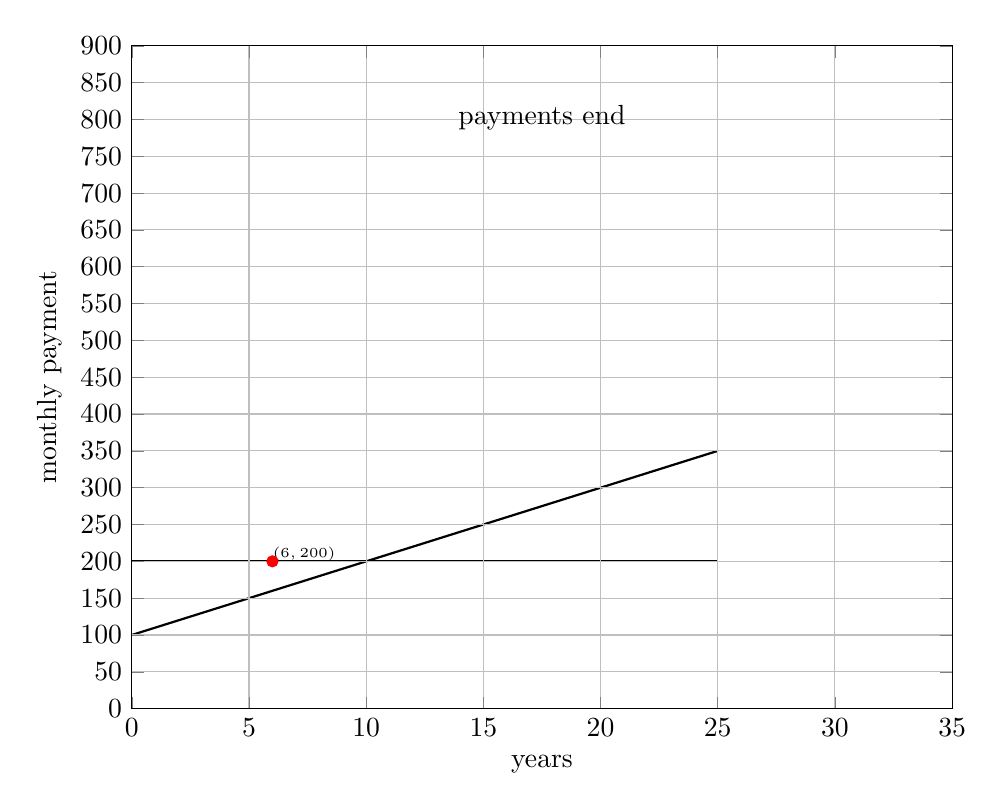
\begin{tikzpicture}
    \begin{axis}[
        width=12cm,
        height=10cm,
        xlabel={years},
        ylabel={monthly payment},
        xmin=0, xmax=35,
        ymin=0, ymax=900,
        xtick={0,5,...,35},
        ytick={0,50,...,900},
        grid=major,
        title style={at={(0.5,0.9)}, anchor=north},
        title={payments end},
        legend pos=north west,
        enlargelimits=false,
        clip=false,
        axis on top,
    ]
    
    % Plot the curve
    \addplot[domain=0:25, samples=100, thick] {150 + 10 * (x - 5)};
    
    % Horizontal line at 200
    \addplot[domain=0:25, samples=2, thick] coordinates {(0,200) (25,200)};
    
    % Red circle at the intersection point
    \addplot[only marks, mark=*, mark size=2pt, color=red] coordinates {(6,200)};
    
    % Text annotation for the intersection point
    \node[anchor=south west, inner sep=0pt] at (axis cs:6,200) {\tiny $(6, 200)$};
    
    \end{axis}
\end{tikzpicture}

\end{document}